
\TVB is logically and technically divided at deploy time into a scientific library and a framework, 
where the scientific library includes datatypes, common analyses and the simulator as its central piece,
while the framework handles execution infrastructure, the web-based user interface and database connectivity. 
While TVB Scientific Library can function independently, as a Python module, TVB Framework needs the scientific library to wrap around it at runtime.

\TVB source code is available for download on Github at \url{https://github.com/the-virtual-brain/}. Previous Git and Python knowledge is required for contributing.
Although you could independently install Python and the rest of TVB dependencies on your machine, and then use the Github code as a local clone, 
we recommend you to download TVB Distribution from \url{http://www.thevirtualbrain.org/register/}, fork our repositories on Github and further use
contributor-setup script from TVB-Distribution to link the two. In this recommended use-case, you will have all TVB Dependencies already installed 
 and under control.

 \begin{figure*}
        \centering
        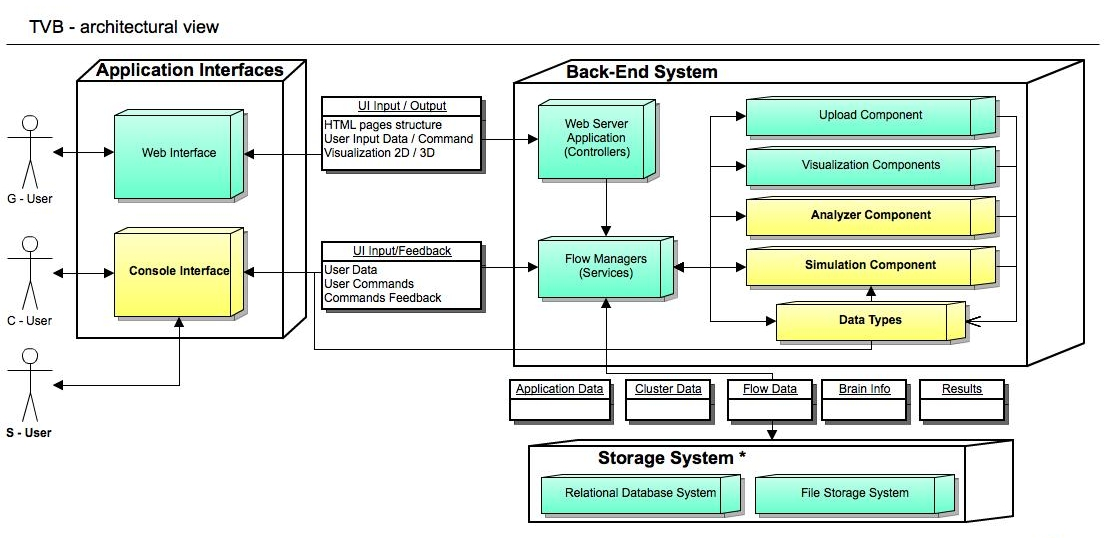
\includegraphics[width=0.90\textwidth]{images/architecture.jpg}
        \caption{\TVB architecture: 
        Yellow blocks are part of the Scientific Library of TVB, while the green blocks are part of TVB Framework.
        TVB provides two independent interfaces, depending on the interaction type wanted by the end-user (web or console).
        TVB Storage layer is compulsory for the web interface, but it can be switched on/off for the console interface.
         }
        \label{fig:architecture}
 \end{figure*}


\subsection{TVB Scientific Library}

	\subsubsection{General description}
TVB Scientific Library code can be found online at \url{https://github.com/the-virtual-brain/scientific_library}

	\subsubsection{Datatypes}


\subsection{TVB Framework}

	\subsubsection{General description}

The framework has been developed with generality and modularity in mind. It
provides a database back-end, workflow management and a number of features to
support collaborative work.  The central idea is data-oriented in a sense that
data are fed and stored into the system and can be transformed into another type
of data (including visualization) through the operation provided by an external
library (including TVB scientific library, but not restricted to it) that have
been \emph{adapted} to the framework. As a consequence, the two central concepts
are \emph{datatypes} i.e. types of data that can be handled in the framework and
\emph{adapters} i.e. processes that allow to interface/adapt external libraries
to  the datatypes handled by within the framework.

The framework also provides user interfaces: web-based graphical interface and
console interface for advanced user and developers.

Due to the generality of the framework, it relies on
the Python \emph{abstract classes} mechanism.
\note[lp]{From Python glossary:}
Abstract base classes complement duck-typing by providing a way to define
interfaces when other techniques like hasattr() would be clumsy or subtly wrong.

\subsubsection{Datatypes}

\paragraph{Description and examples}

\note[lp]{From FIN paper:} TVB-datatypes are annotated data structures which
contain one or more data attributes and associated descriptive information, as
well as methods for operating on the data they contain. The definition of a
datatype is achieved using TVB's traiting system, which was inspired by the
traiting system developed by Enthought \cite{Enthought_2001} 

\note[lp]{The TVB-trait system might be worth described here?}

\note[lp]{Table 2 "TVB datatypes" of FIN article might be interesting here?}

In scientific Python code, it is conventional to provide arguments
of an algorithm as a "bare" array or collection there of, and sanity
checks of arguments proceed on the basis of array geometry, for example.
In \TVB, we consider a \textit{datatype} to be a full, formal description of 
an entity involved in an algorithm that would be part of \TVB. 
For example, the \texttt{Connectivity} datatype, which may elsewhere
be represented by a simple $N$ by $N$ NumPy array, is written as a class
in which one of the attributes, \texttt{weights} is a explicitly typed 
\texttt{FloatArray}, and the declaration of this type is complemented by
explicit label, default values, and documentation strings. 

\note[mw]{Add a listing showing this}.

Because an explicit goal of \TVB was to provide a user interface to each of the
datatypes and algorithms contained within, it is necessary at some point to
provide metadata. A \texttt{traits} system was developed, similar to that of
IPython or EPD, was developed, allowing for a attributes of a datatype class to
be written out with full metadata. An extensive set of existing building 
blocks are already provided from numeric types and arrays to lists, tuples, 
string, and dictionaries.

\note[mw]{Show description of a data type}

 When methods of such a class are invoked,
they may use the traited attributes directly, accessing either a default value
or one given during the instantiation of the object. Additionally, this allows
the web-based UI to introspect a class for all of its attributes and their
descriptions, to provide help in the interface. The explicit typing also allows
such classes to be nearly automatically mapped to SqlAlchemy \& HDF5 tables,
the combination of which provides persistence for datatypes when using the web
UI.  Lastly, because such metadata is used to build the docstring of a class,
the IPython user also may obtain extensive descriptions of attributes and
function arguments in the usual way. 

\note[lp]{The Connectivity datatype might be an example}

\paragraph{Datatypes, data storage and retrieval} 

Data storage is managed using \emph{SQLAlchemy}
\texttt{http://www.sqlalchemy.org/} which provides a common interface for the
two proposed storage system: SQLite and PostgreSQL \note[lp]{or flat file
system?}.

\subsubsection{Adapters}

\paragraph{General description}

While datatypes provide a way of description what algorithms work with, 
sufficing for the typical user looking to write scripts against the
available libraries, the web-based UI requires algorithms to adhere to 
a generic interface, which is elsewhere referred to as the Adapter pattern.
Typically, this implies that a class is written that is able to describe
the collection to datatypes required and a single method to invoke the
algorithm.

Adapters are derived from the abstract class named \texttt{ABCAdapter} which
defines the common interface for the adapters with methods...

Several categories of adapters have been defined: 
\begin{itemize}
    \item \textit{analyzers} which allow the interface between libraries
        containing algorithm for the analysis of the data (wavelets, FastICA,
        etc.) and the TVB framework and datatypes.
    \item \textit{creators}
    \item \textit{exporters} 
    \item \textit{portlets} 
    \item \textit{simulator}
\item \textit{uploaders}: allow the upload of external data into TVB framework
    such as gifti files of plain csv files.
\item \textit{visualizers} \note[lp]{derived from the ABCDisplayer abstract class} allow
    to display the correct datatype.
\end{itemize}


\note[mw]{Show the adapter for FastICA}

Note that the adapters and datatypes are intended to provide full 
power and flexibility of the framework; when the simulator is invoked from
the web-based UI, it is done so through an \texttt{SimulatorAdapter} which,
despite being relatively complex, is datatypes all the way down.

It is reasonable to ask to what such a scheme offers over the more 
conventional approach of Python, where presumably it would have been
sufficient that each adapter consist of a class with an \texttt{\_\_init\_\_}
and \texttt{\_\_call\_\_} method, in the case of a function type. 
We note that because in the case of \TVB, the context in which an object
is used is more varied, e.g. not simply initialized but loaded through 
SqlAlchemy's ORM, and that the adapter is required to perform more tasks
than just initialization and invocation, e.g. provide expected shape of 
result, it was advantageous to create a distinct set of interfaces built
on the abstract base class framework provided by Python's standard library.

\paragraph{Adapting sklearn's FastICA}

\paragraph{Interfacing with MATLAB}

One of the well-known libraries for characterizing anatomical 
and functional connectivity is the Brain Connectivity Toolbox. Because
it is written in MATLAB, with maintainers who prefer MATLAB, we 
chose not to port routines of the library to Python but instead use
a MATLAB adapter which runs arbitrary MATLAB code. This generic
adapter works by generating a wrapper script for the MATLAB code, which
wraps the code in a try-except clause, and loads and saves the workspace
before and after execution, 
generating a workspace \texttt{.mat} file, invoking the MATLAB or Octave
executable, and loading the resulting workspace file. Despite invocation
of MATLAB being a relatively slow operation, this works fine in a single
user situation, and where Octave is available, it is quite fast. In the 
case that many operations are necessary, they can be batched into the 
same run.


